
\documentclass[a4paper, 12pt]{article}
\usepackage[T1]{fontenc}
\usepackage{times}
\usepackage[swedish]{babel}
\usepackage[utf8]{inputenc}
%\usepackage{dtklogos}
\usepackage{wallpaper}
\usepackage[absolute]{textpos}
\usepackage[top=2cm, bottom=2.5cm, left=3cm, right=3cm]{geometry}
\usepackage{appendix}
\usepackage[nottoc]{tocbibind}
\setcounter{secnumdepth}{3}
\setcounter{tocdepth}{3}
\usepackage{sectsty}
\sectionfont{\fontsize{14}{15}\selectfont}
\subsectionfont{\fontsize{12}{15}\selectfont}
\subsubsectionfont{\fontsize{12}{15}\selectfont}
\usepackage{csquotes} 
\renewcommand{\thetable}{\arabic{section}.\arabic{table}}  
\renewcommand{\thefigure}{\arabic{section}.\arabic{figure}} 
\usepackage{amsmath}
\usepackage{algorithm}
\usepackage[noend]{algpseudocode}

\usepackage{listings}
\usepackage{lstlang}


\newsavebox{\mybox}
\newlength{\mydepth}
\newlength{\myheight}
\newenvironment{sidebar}
{\begin{lrbox}{\mybox}\begin{minipage}{\textwidth}}
{\end{minipage}\end{lrbox}
 \settodepth{\mydepth}{\usebox{\mybox}}
 \settoheight{\myheight}{\usebox{\mybox}}
 \addtolength{\myheight}{\mydepth}
 \noindent\makebox[0pt]{\hspace{-20pt}\rule[-\mydepth]{1pt}{\myheight}}
 \usebox{\mybox}}

\newcommand\BackgroundPic{
    \put(-2,-3){
    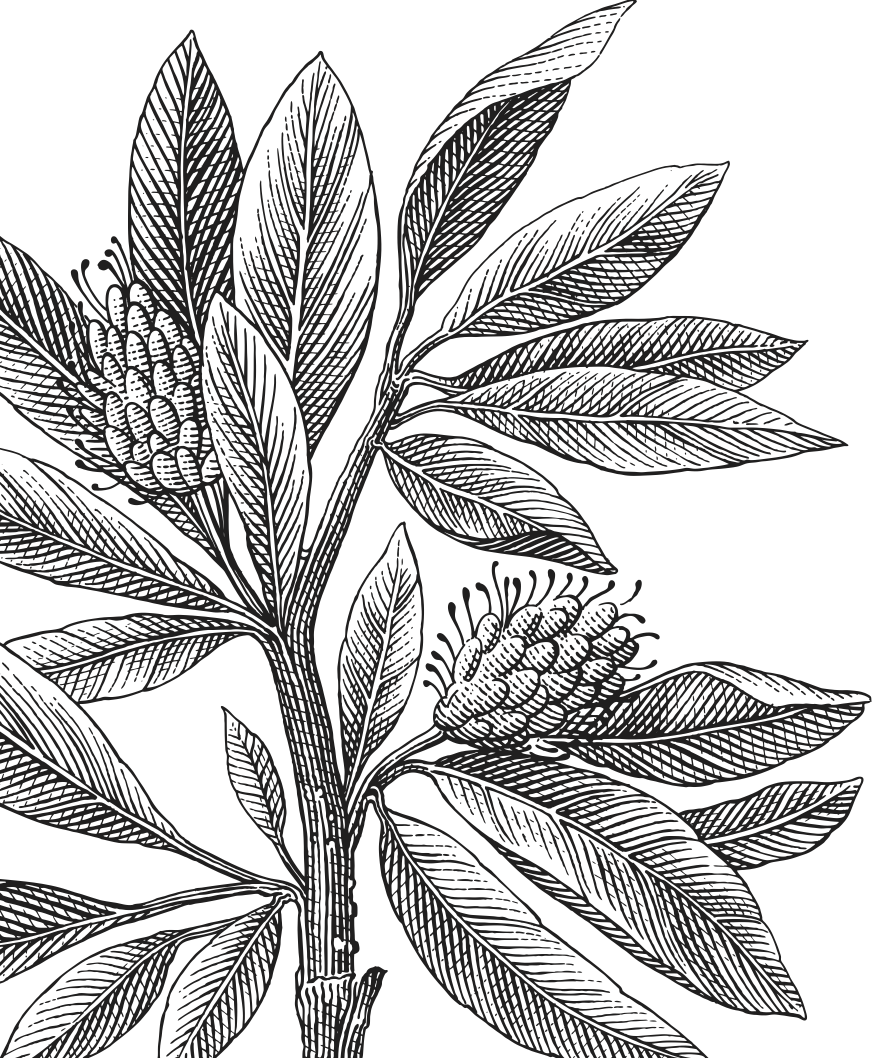
\includegraphics[keepaspectratio,scale=0.3]{lnu_etch.png} 
    }
}
\newcommand\BackgroundPicLogo{
    \put(30,740){
	
\includegraphics[keepaspectratio,scale=0.10]{logo.png}     
    }
}
\definecolor{MyDarkGreen}{rgb}{0.0,0.4,0.0} % This is the color used for comments
\lstloadlanguages{AVR}%
\lstset{language=AVR, % AVR 8-bit Assembler
        frame=single, % Single frame around code
        basicstyle=\small\ttfamily, % Use small true type font
        keywordstyle=\color{Blue}\bf, % Instructions in blue, bold
        keywordstyle=[2]\color{Orange}, % Registers and ports in orange
        keywordstyle=[3]\color{Purple}, % Directives in purple
        commentstyle=\usefont{T1}{pcr}{m}{sl}\color{MyDarkGreen}\small,
        tabsize=5, % 5 spaces per tab
        numbers=left, % Line numbers on left
        firstnumber=1, % Line numbers start with line 1
        numberstyle=\tiny\color{Blue}, % Line numbers are blue and small
        stepnumber=5 % Line numbers go in steps of 5
        }

% Creates a new command to include an asm script,
% the first parameter is the filename of the program (without .asm),
% the second parameter is the caption
\newcommand{\avrasm}[2]{
\begin{itemize}
\item[]\lstinputlisting[caption=#2,label=#1]{#1.asm}
\end{itemize}
}



%\usepackage[backend=bibtex,bibencoding=ascii,style=authoryear,sorting=none]{biblatex}

\title{	
\vspace{-8cm}
\begin{sidebar}
    \vspace{5cm}
    \normalfont \normalsize
    \Huge Rapport \\
    \vspace{-1.3cm}
\end{sidebar}
\vspace{3cm}
\begin{flushleft}
    \huge Laboratory Report\\  
\end{flushleft}
\null
\vfill
\begin{textblock}{6}(10,13)
\begin{flushright}
\begin{minipage}{\textwidth}
\begin{flushleft} \large
	\emph{Author:} Caroline Nilsson \\ Daniel Alm Grundström \\
	%\emph{Handledare:} \\ 
	\emph{Termin:} HT 2017\\ 
	\emph{Course:} 1DT301 - Computer Technology I\\
\end{flushleft}
\end{minipage}
\end{flushright}
\end{textblock}
}
\date{\today} 



\begin{document}
\pagenumbering{gobble}
\newgeometry{left=5cm}
\AddToShipoutPicture*{\BackgroundPic}
\AddToShipoutPicture*{\BackgroundPicLogo}
\maketitle
\restoregeometry
\clearpage



\pagenumbering{gobble}

\tableofcontents
\newpage
\pagenumbering{arabic}



\section{Introduktion}
In the process of working with the laboratory assignments we started by doing research about the assembly language and the STK600 in order to better understand how to solve the different assignments. 
In each assignment we first created a pseudocode solution which we converted to flowchart diagrams, then it was rather simple to convert this into assembly language. Common for all assignments is also that we have been using the simulations to confirm that the program is working and completing the correct tasks. 

\newpage
\section{Assignment 1}
In the first assignment we were to light up Led2 (which is the third light counting from the right). 

\begin{algorithm}
\caption{Light Led2}
\label{Assign.1 Pseudo}
\begin{algorithmic}
\Procedure{Pseudocode}{}
\State{$PortB = output$}
\State{$Led2\ bitstring \rightarrow PortB$}
\State{$Repeat\ step\ 2$} 
\EndProcedure
\end{algorithmic}
\end{algorithm}

\begin{figure}[h]
\label{assign1.flow}
\caption{Flowchart}
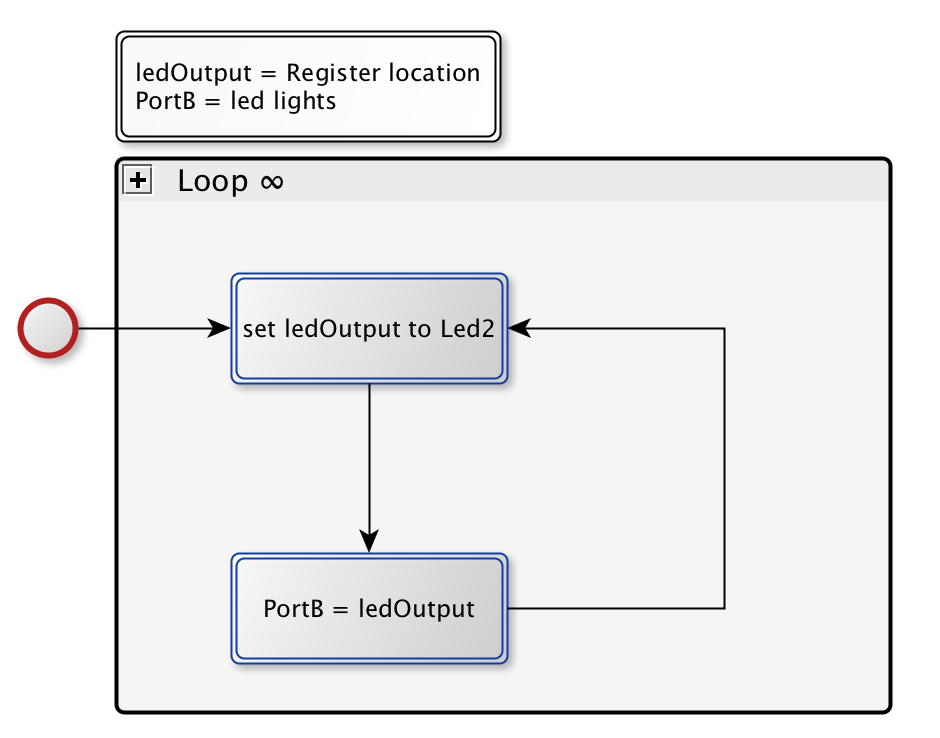
\includegraphics[scale=0.5]{Flowchart_pics/assignment1_pic.png} 

\end{figure}

The pseudocode and the flowchart shows that we first set Port B as an output port, the value 0000 0100 is saved at a register location (in our case that is R16) and then sent to Port B which makes Led2 (or the third light from the right) light up. 
Minimum lines of code?



\newpage

\section{Assignment 2}

\newpage

\section{Assignment 3}

\newpage

\section{Assignment 4}

\newpage

\section{Assignment 5}

\newpage

\section{Assignment 6}

\newpage


\pagenumbering{Alph}
\setcounter{page}{1} 
\appendix
\section{Bilaga 1} 

\end{document}